\subsection{Reengineered Task Organization Model}
Das Reengineered Task Organization Model repräsentiert die Arbeit der Benutzer mithilfe des zu entwicklende System. Die Abbildung \ref{img:reengineeredTaskOrganizationModel}: \nameref{img:reengineeredTaskOrganizationModel} beschreibt den Prozess der Arbeit des Diabetikers mit dem System anhand der Concrete Use Cases aus der Aufgebenmodellierung und ergänzt das Task Organization Model. Alle Erkenntisse aus der Aufgabenmodellierung fließen zunächst in das Reengineered Task Organization Model und folglich auch in das Design der Screens ein.
\begin{figure}[H]
	\centering
	\setlength{\fboxsep}{1pt}
	\setlength{\fboxrule}{1pt}
	\fbox{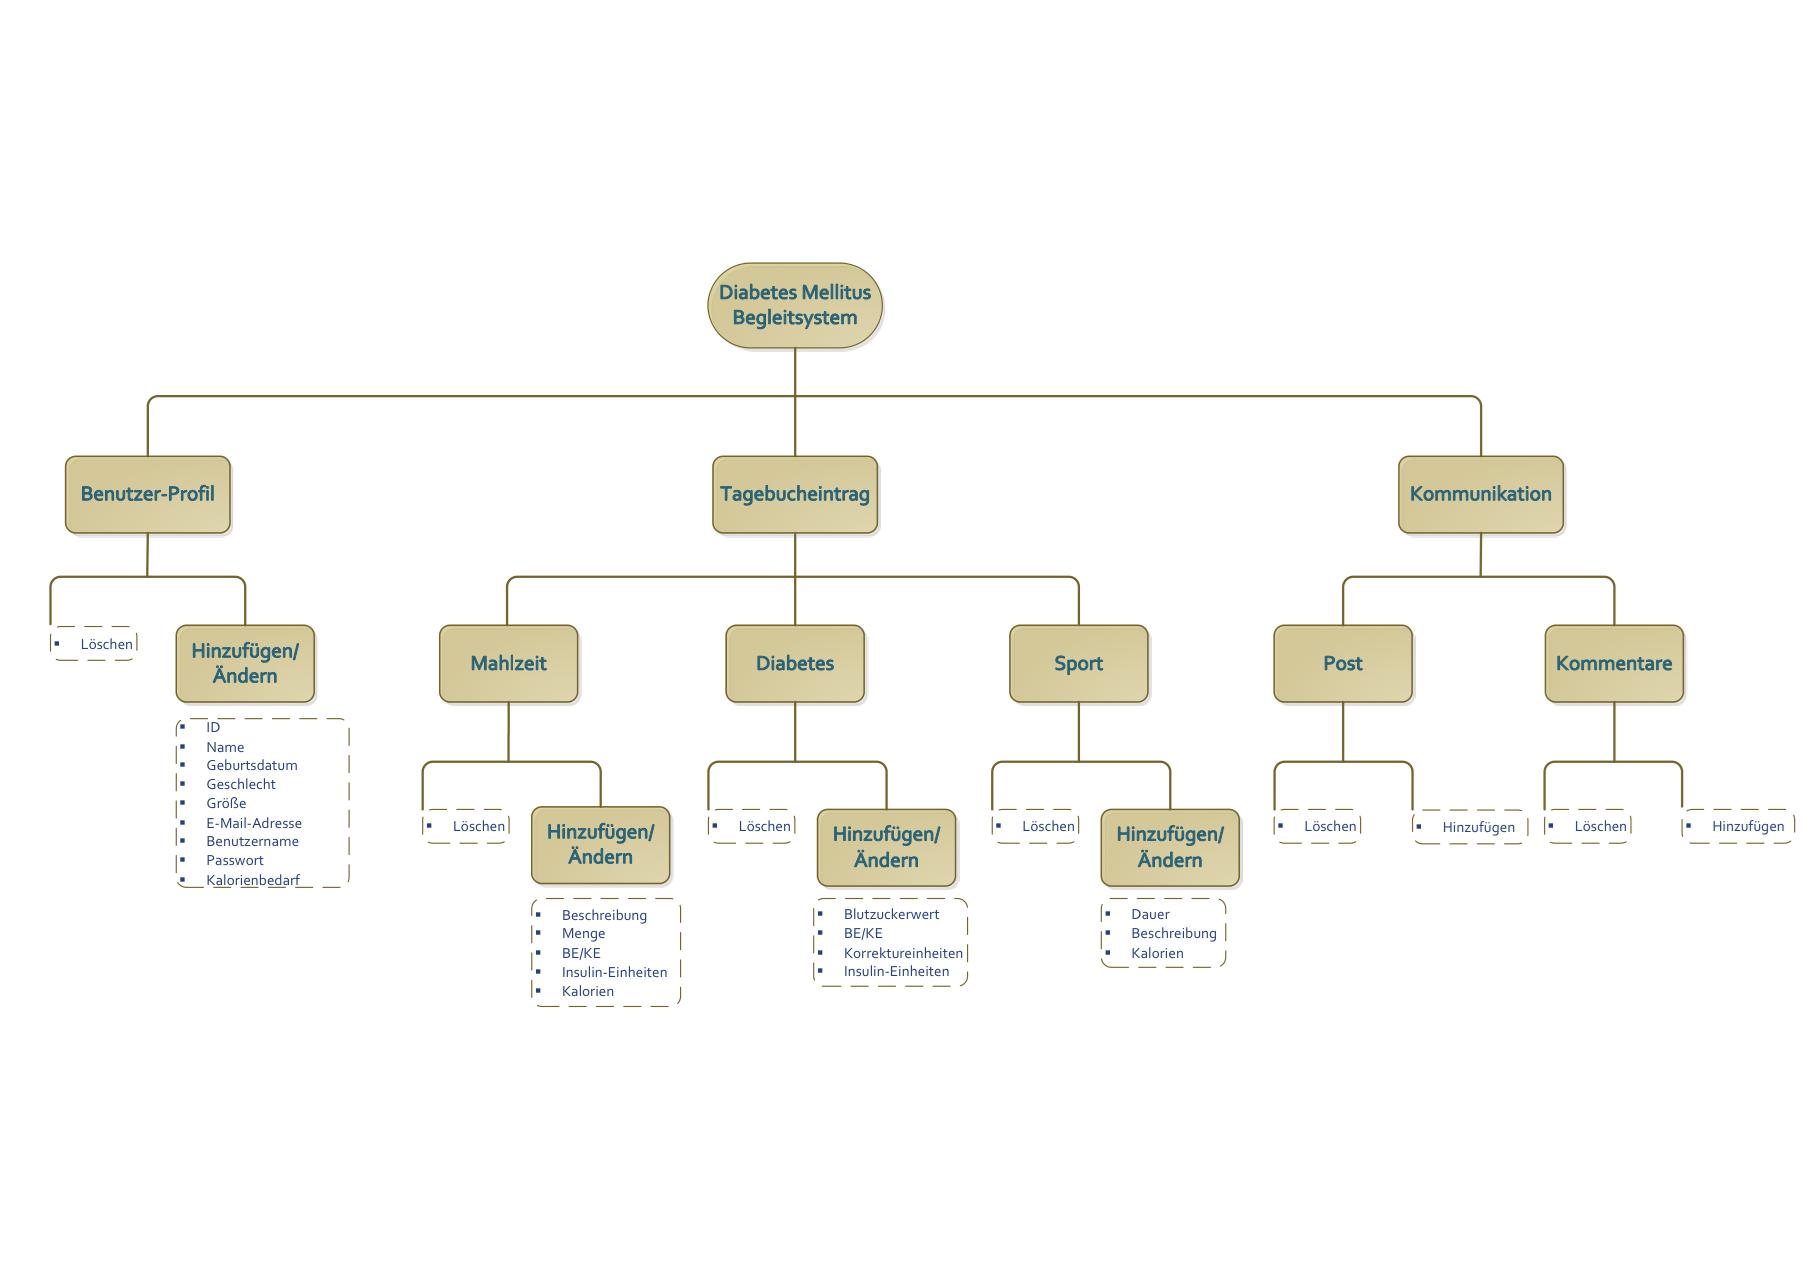
\includegraphics[width=1.0\textwidth]{images/reengineeredTaskOrganizationModel.png}}
	\captionsetup{justification=centering}
	\caption{Reengineered Task Organization Model}
	\label{img:reengineeredTaskOrganizationModel}
\end{figure}
\subsection{Conceptual Model (CM) Design}
Im Concetpual Model Design werden erste Screens für das zu entwickelnde System designt. Die ersten groben Entwürfe sollen den Navigationspfad und die Haupt-Screens identifizieren und anhand dessen erste Regeln für das finale Design des Interfaces festlegen. Ziel ist hier jedoch nicht ein detailreiches Interface Design zu bestimmen. Dieses Design muss zunächst in den kommenden Designaufgaben entwickelt werden.\\
Nach Mayhew \cite{MD} muss zunächst bestimmt werden, ob es sich bei dem Conceputal Model Design um ein product- oder process-oriented model handelt. Da es in dem zu entwickelnde System keine Arbeitsprodukte, welche vom Benutzer individuell erstellt oder bearbeitet werden. In diesem System sollen die Arbeitsprozesse von Diabetikern unterstützt werden. Auf Informationen wie die Nährwerte von Lebensmitteln haben alle Benutzer Zugriff, können abgerufen und in ihrem Tagebuch gespeichert werden. Aufgrund dessen handelt es sich in diesem Fall um ein process-oriented model.\\
In nächsten Schritt sind die Prozesse des process-oriented model zu identifizieren. Bei einem process-oriented model definiert das \nameref{img:reengineeredTaskOrganizationModel} auf Seite \pageref{img:reengineeredTaskOrganizationModel} die (Unter-)Prozesse des Systems und aus diesem lässt sich folgende Aufgabenhierarchie ableiten:\\
Benutzer\newline
\noindent\hspace*{10mm}Benutzer hinzufügen\newline
\noindent\hspace*{10mm}Benutzer bearbeiten\newline
\noindent\hspace*{10mm}Benutzer löschen\newline
Tagebuch\newline
\noindent\hspace*{10mm}Blutzuckerwert\newline
\noindent\hspace*{20mm}Blutzuckerwert hinzufügen\newline
\noindent\hspace*{20mm}Blutzuckerwert bearbeiten\newline
\noindent\hspace*{20mm}Blutzuckerwert löschen\newline
\noindent\hspace*{10mm}Mahlzeit\newline
\noindent\hspace*{20mm}Mahlzeit hinzufügen\newline
\noindent\hspace*{20mm}Mahlzeit bearbeiten\newline 
\noindent\hspace*{20mm}Mahlzeit löschen\newline
\noindent\hspace*{10mm}Aktivität\newline
\noindent\hspace*{20mm}Aktivität hinzufügen\newline
\noindent\hspace*{20mm}Aktivität bearbeiten\newline
\noindent\hspace*{20mm}Aktivität löschen\newline
Kommunikation\newline
\noindent\hspace*{10mm}Beitrag\newline
\noindent\hspace*{20mm}Beitrag hinzufügen\newline
\noindent\hspace*{20mm}Beitrag löschen\newline
\noindent\hspace*{10mm}Kommentar\newline
\noindent\hspace*{20mm}Kommentar hinzufügen\newline
\noindent\hspace*{20mm}Komentar löschen\\
Um nun die Darstellungregeln für die Prozesse zu gestalten wird eine Bottom-Navigation-Bar verwendet. Die Navigation könnte wie in Abbildung \ref{img:navigationbar}: \nameref{img:navigationbar} dargestellt werden. \newline
Für eine Bottom-Navigation-Bar wurde sich entschieden, um den Benutzer Kontrolle über das System und eine gewisse Freiheit zu gewährleisten. So ermöglicht das System dem Benutzer bei versehentlicher Auswahl einer Navigation einen deutlich gekennzeichneten „Notausgang“, indem der Benutzer lediglich durch die Bottom-Navigation den unerwünschten Systemzustand verlässt, ohne einen erweiterten Dialog durchlaufen zu müssen.
\begin{figure}[H]
	\centering
	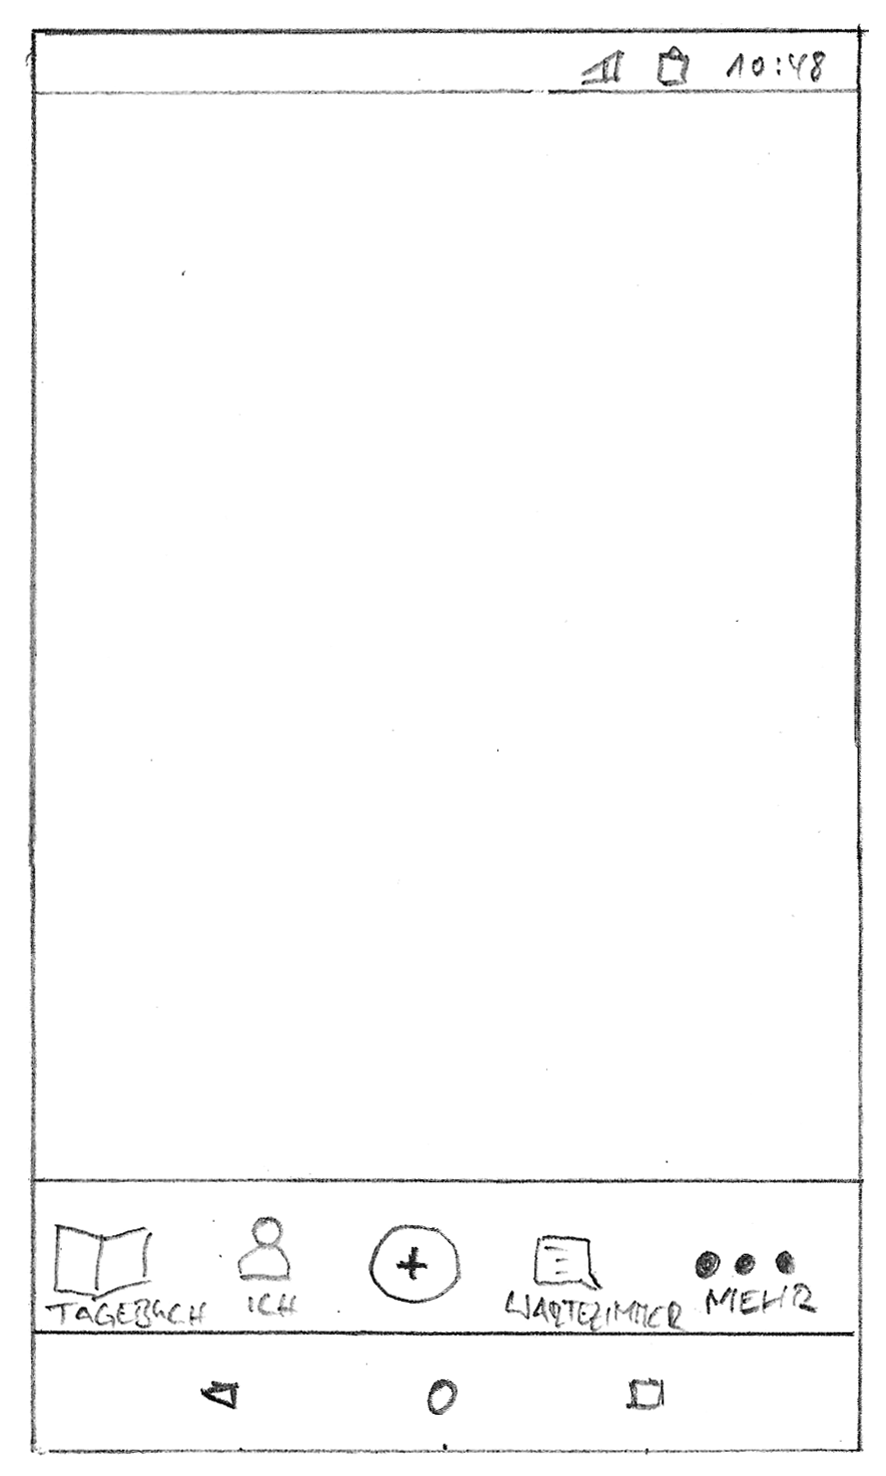
\includegraphics[width=0.35\textwidth]{images/navigationbar.png}
	\captionsetup{justification=centering}
	\caption{Bottom-Navigation-Bar}
	\label{img:navigationbar}
\end{figure}
Unter dem Navigationspfad „Tagebuch“ (Abbildung \ref{img:tagebuchscreen}: \nameref{img:tagebuchscreen})sind Blutzuckerwerte, Mahlzeiten und Aktivitäten anzulegen, zu bearbeiten, einzusehen und zu löschen. Unter „Ich“ (Abbildung \ref{img:ichscreen}: \nameref{img:ichscreen}) und „Mehr“ (Abbildung \ref{img:mehrscreen}: \nameref{img:mehrscreen}) können Benutzerkonten eingesehen, bearbeitet und gelöscht werden und im „Wartezimmer“ (Abbildung \ref{img:wartezimmerscreen}: \nameref{img:wartezimmerscreen}) sind Beiträge und Kommentage einzusehen, hinzuzufügen und zu löschen. Das Plus-Icon ermöglich zusätzlich das hinzufügen von Blutzuckerwerten, Mahlzeiten, Aktivitäten und Beiträge. So könnten die Screens folgendermaßen dargestellt werden. 
\begin{figure}[H]
	\centering
	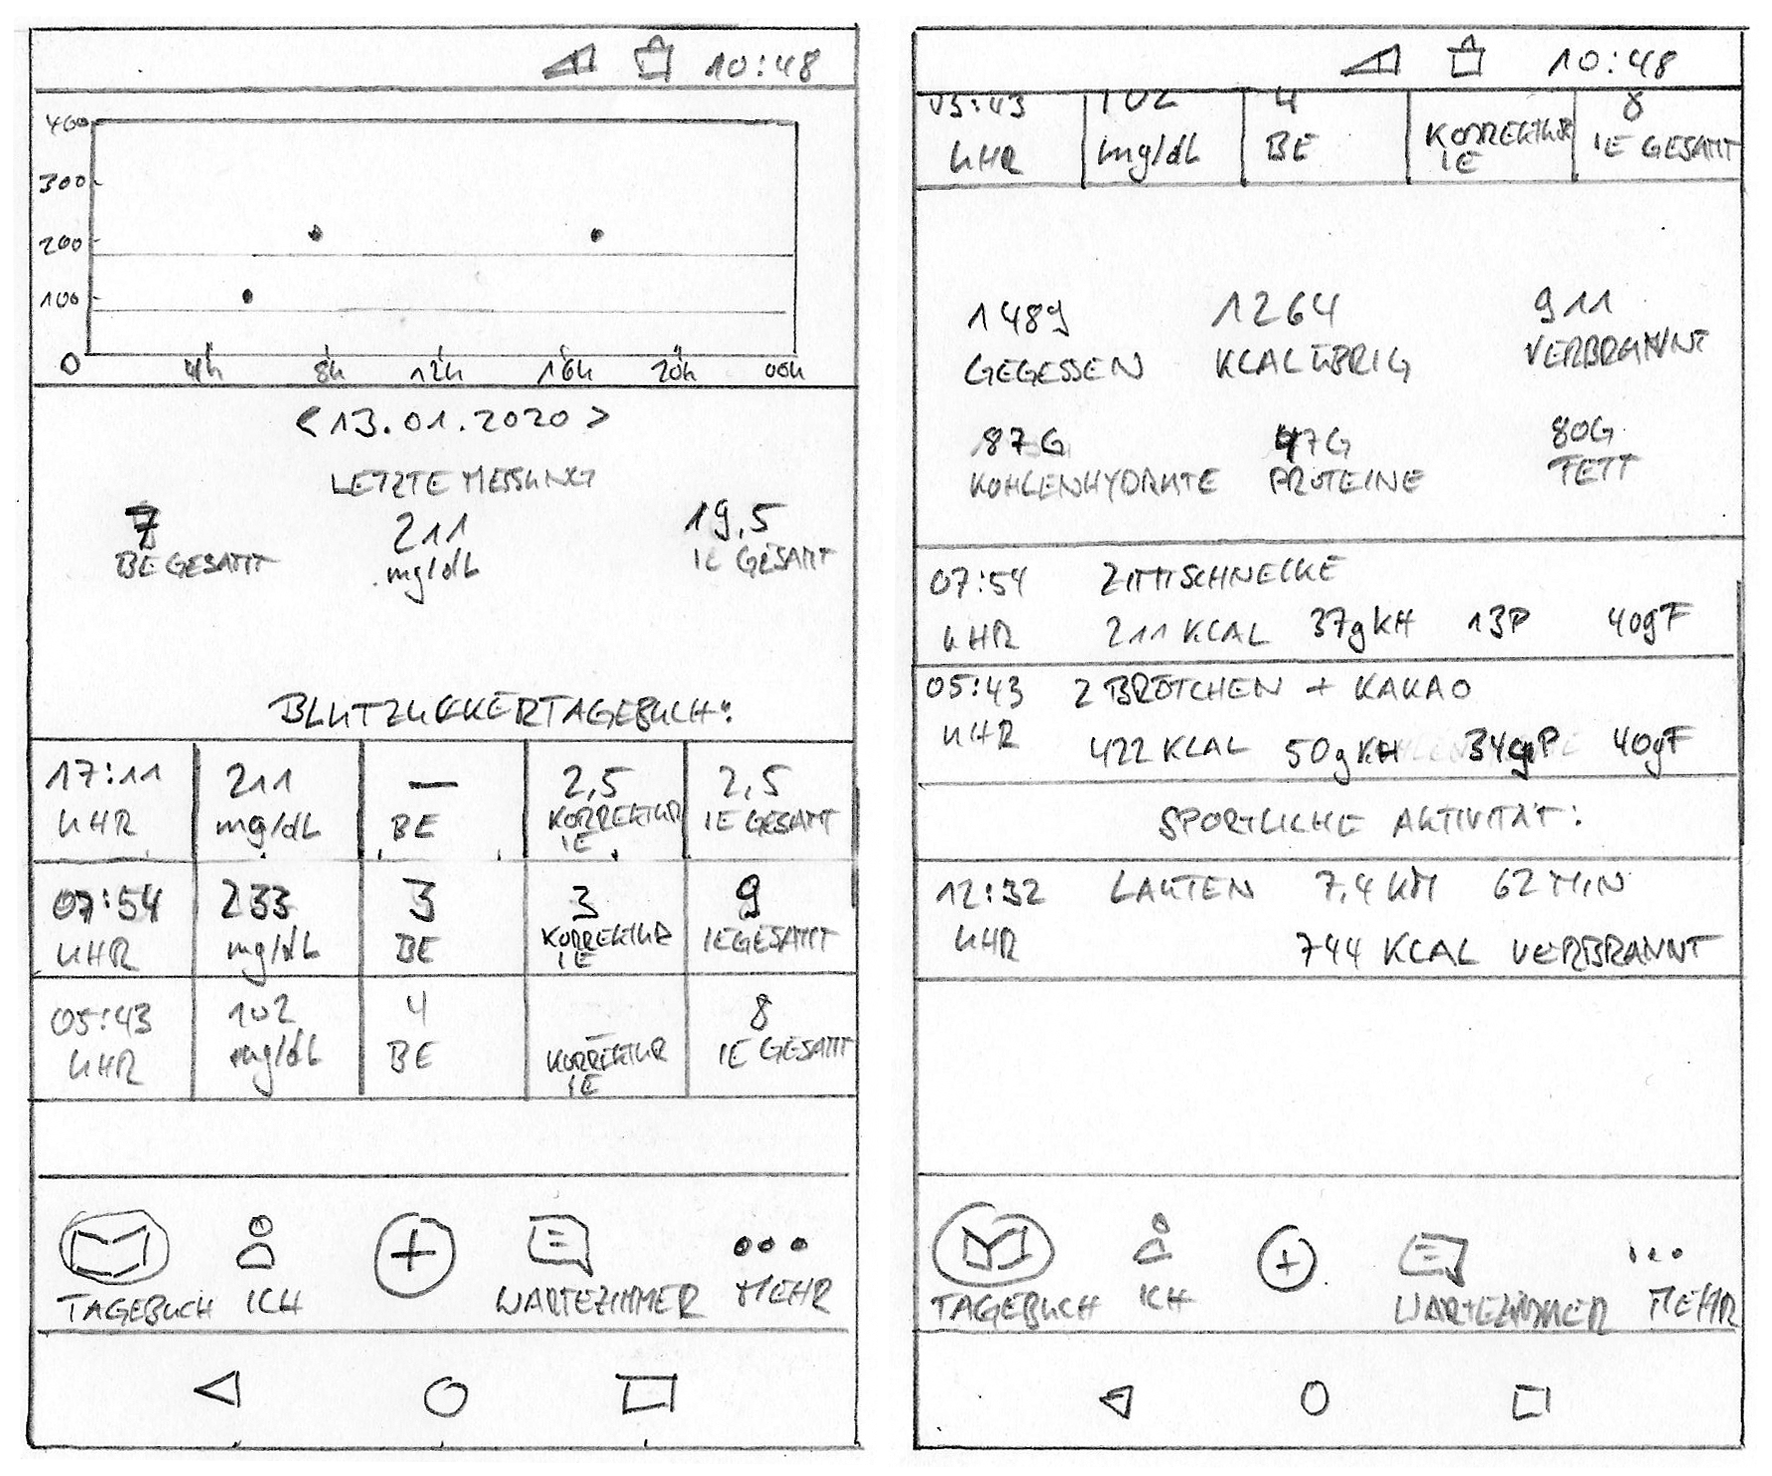
\includegraphics[width=0.7\textwidth]{images/tagebuchscreen.png}
	\captionsetup{justification=centering}
	\caption{Tagebuch-Screen}
	\label{img:tagebuchscreen}
\end{figure}
\begin{figure}[H]
	\centering
	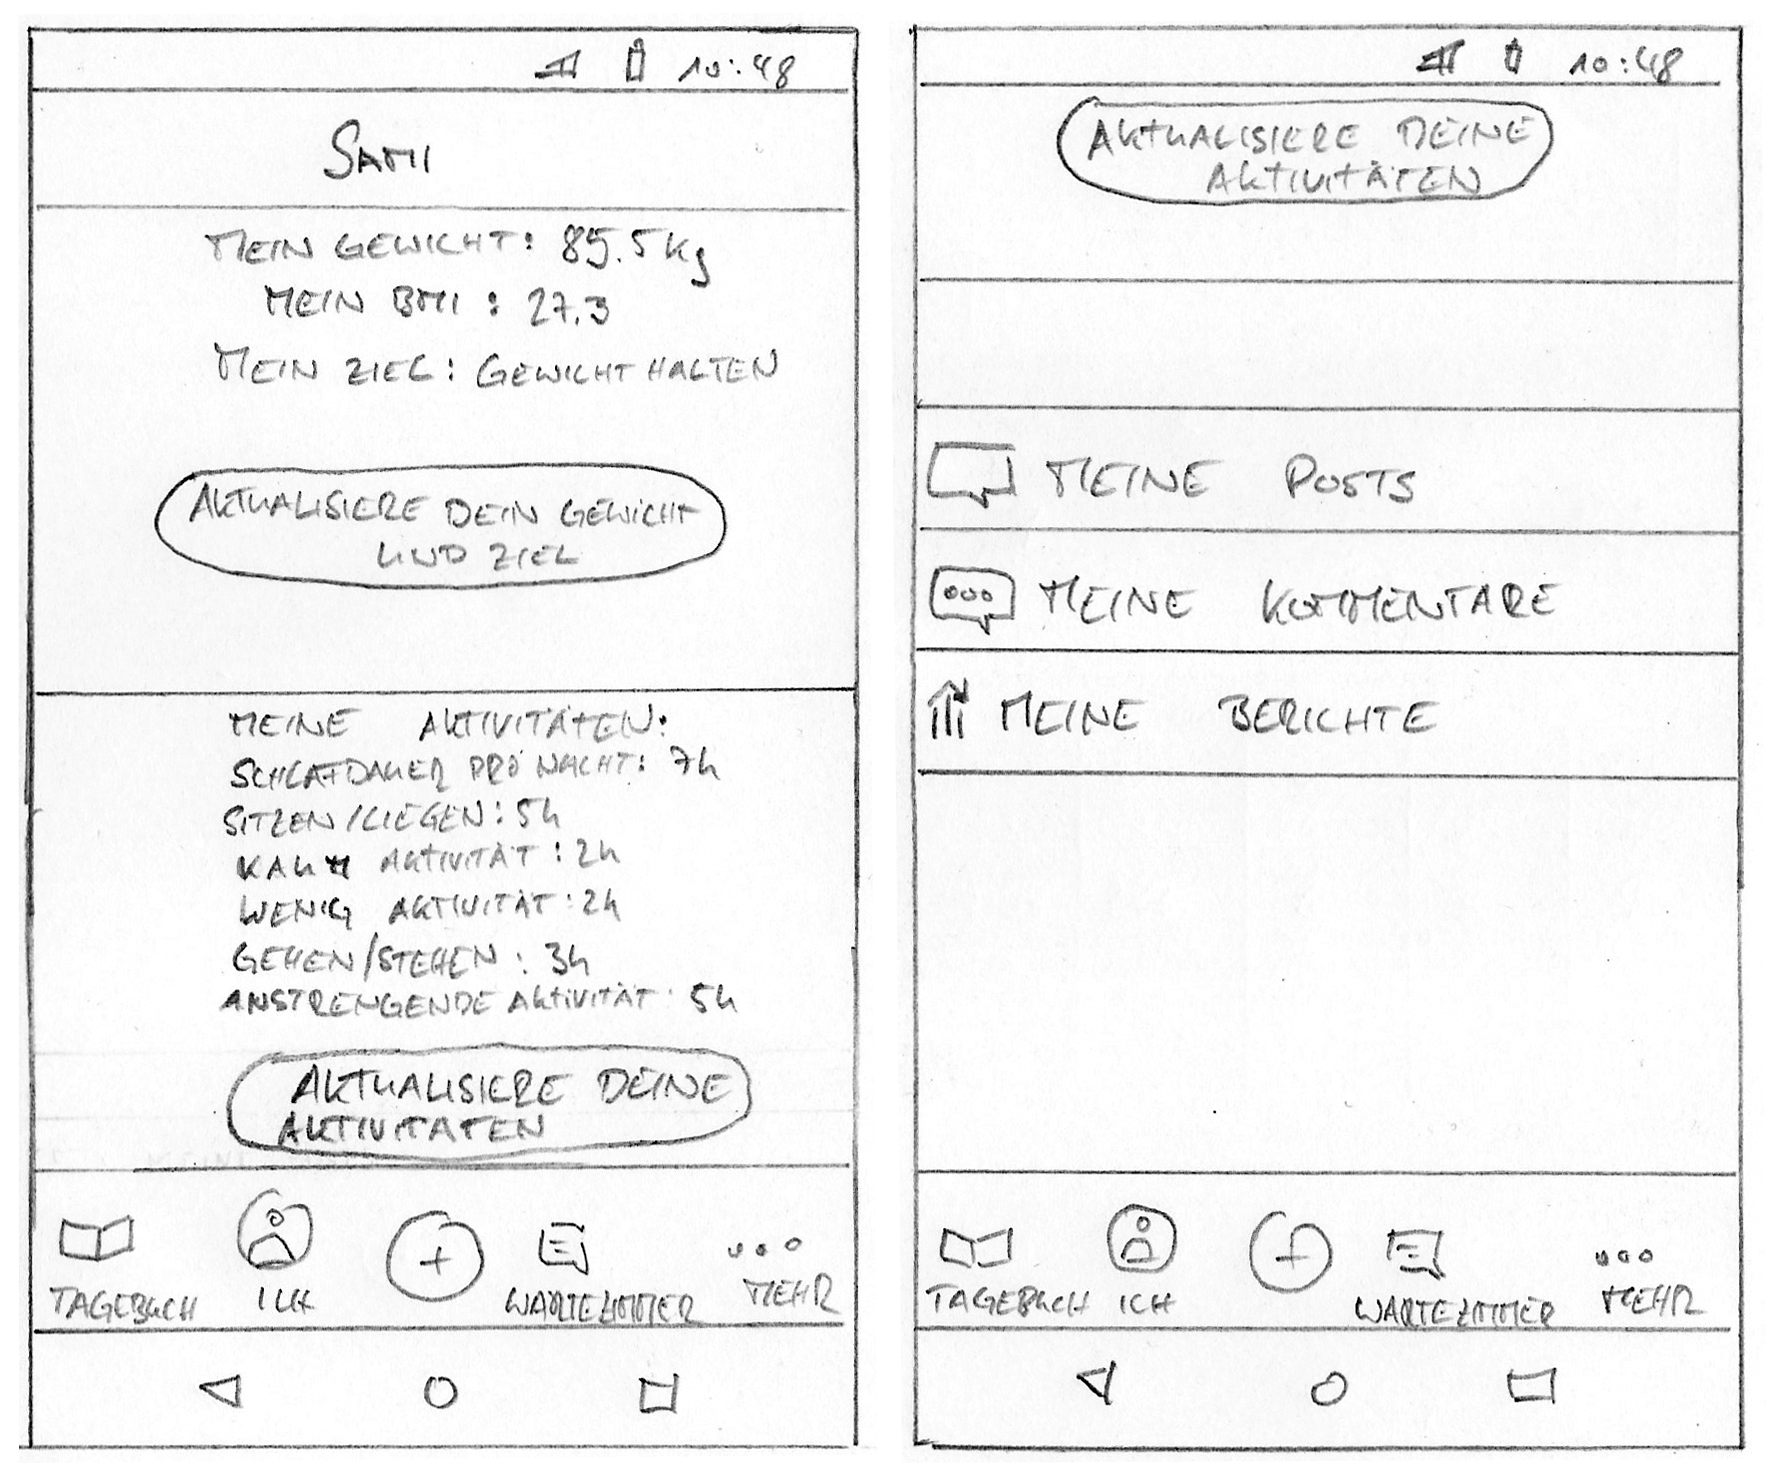
\includegraphics[width=0.7\textwidth]{images/ichscreen.png}
	\captionsetup{justification=centering}
	\caption{Ich-Screen}
	\label{img:ichscreen}
\end{figure}
\begin{figure}[H]
	\centering
	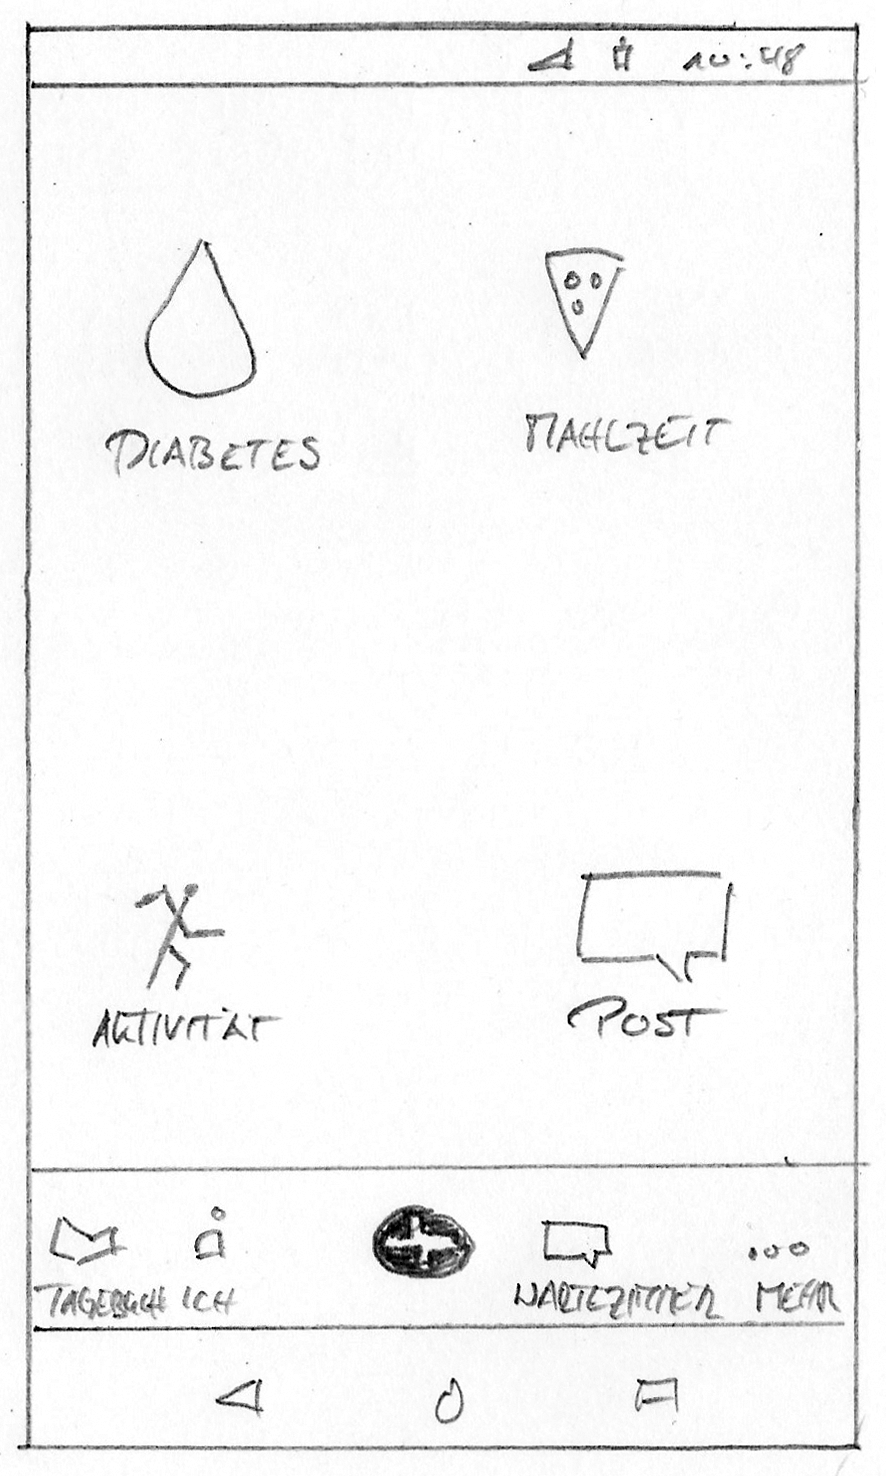
\includegraphics[width=0.35\textwidth]{images/addscreen.png}
	\captionsetup{justification=centering}
	\caption{Add-Screen}
	\label{img:addscreen}
\end{figure}
\begin{figure}[H]
	\centering
	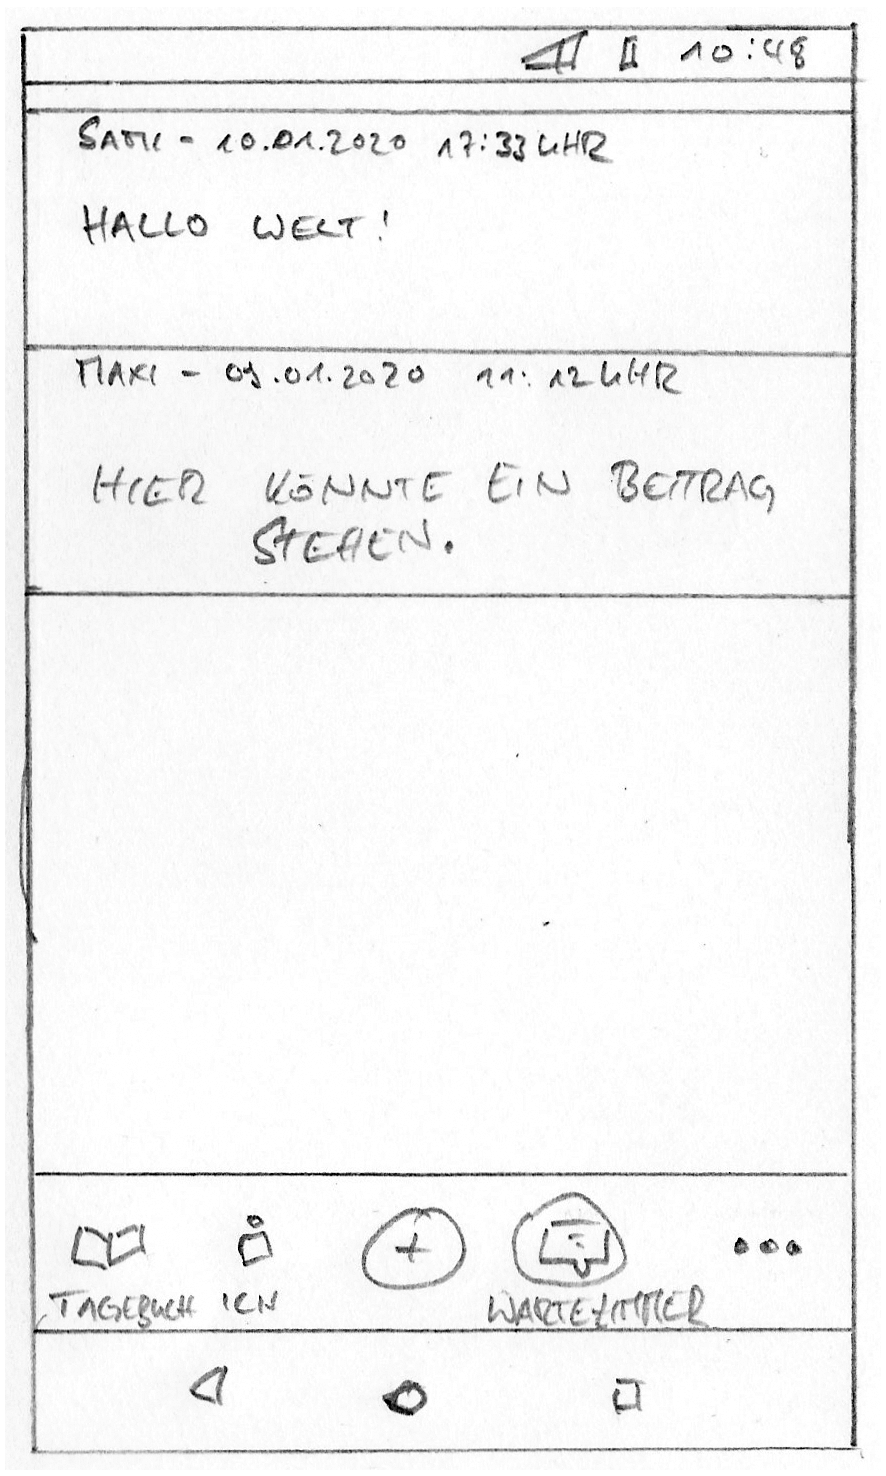
\includegraphics[width=0.35\textwidth]{images/wartezimmerscreen.png}
	\captionsetup{justification=centering}
	\caption{Wartezimmer-Screen}
	\label{img:wartezimmerscreen}
\end{figure}
\begin{figure}[H]
	\centering
	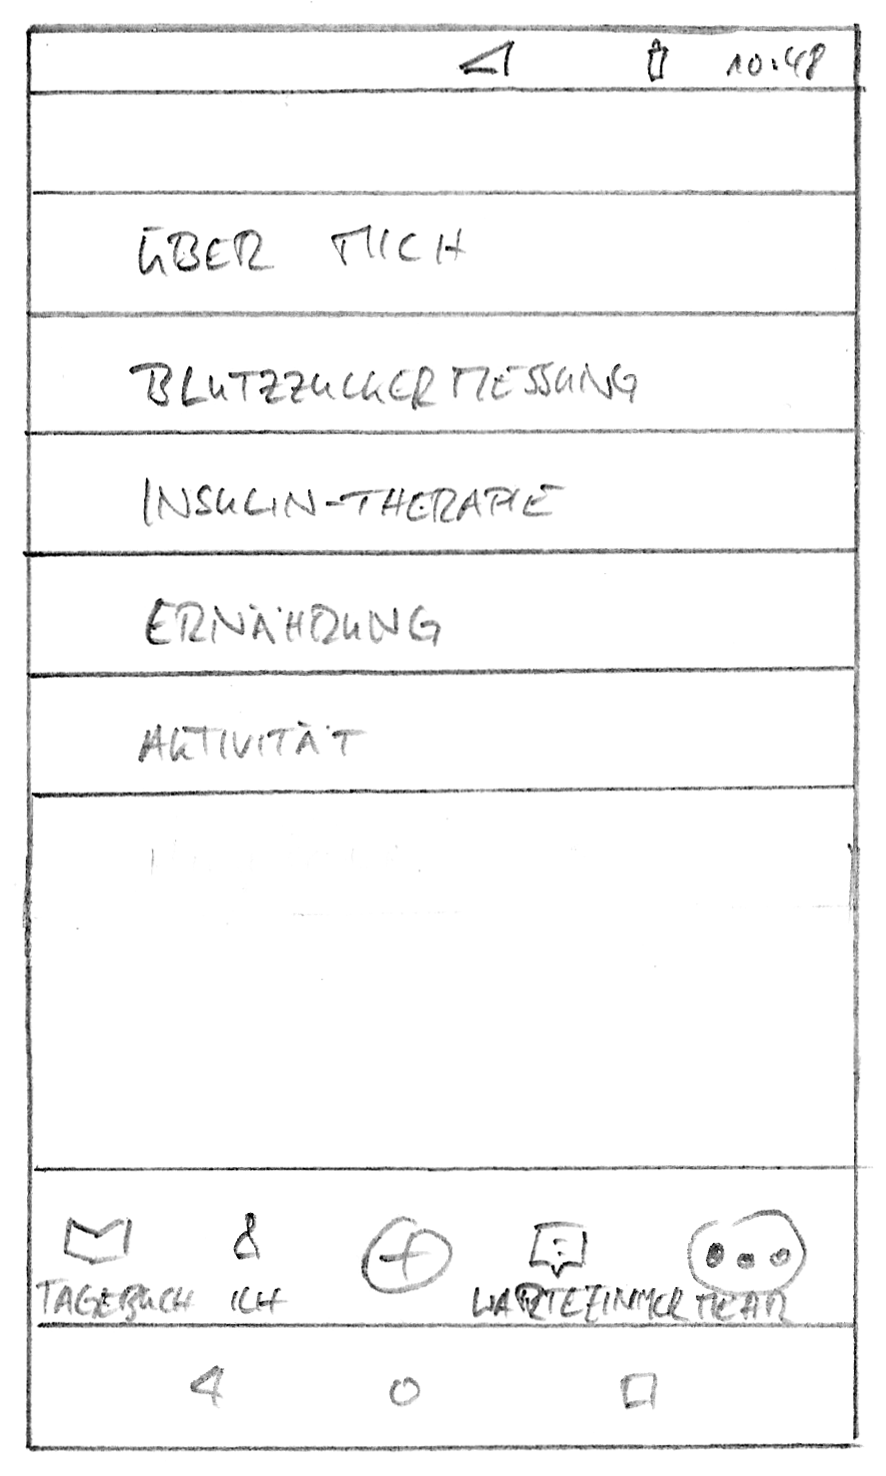
\includegraphics[width=0.35\textwidth]{images/mehrscreen.png}
	\captionsetup{justification=centering}
	\caption{Mehr-Screen}
	\label{img:mehrscreen}
\end{figure}
Die Begriffswahl für „Tagebuch“ (Abbildung \ref{img:tagebuchscreen}: \nameref{img:tagebuchscreen}) ensteht aus der Domäne, das Diabetiker „Tagebucheinträge“ verfassen.  „Ich“ (Abbildung \ref{img:ichscreen}: \nameref{img:ichscreen}) repräsentiert benutzerbezogene Daten und „Wartezimmer“ (Abbildung \ref{img:wartezimmerscreen}: \nameref{img:wartezimmerscreen} ist eine metaphorische Bezeichnung für eine Treffpunkt verschiedener Benutzer. Unter „Mehr“ (Abbildung \ref{img:mehrscreen}: \nameref{img:mehrscreen}) sind wiederum benutzerbezogene Einstellungen zu bearbeiten. Durch die verschiedenen Navigationspfade soll der Benutzer durch stets angemessene Informationen innerhaln angemessener Zeit auf dem Laufenden gehalten werden.\\
Nach dem Conceputal Model Design folgt das Conceptual Model Mock-Up und die Iterative Conceptual Model Evaluation, in denen die ersten Entwürfe eines Designs mit Stift und Papier erstellt  und anhand von Probanden evaluiert werden. Da allerdings gibt der begrenzte Zeitrahmen diese zwei Arbeitschritte nicht her, wodurch die Abbildungen als Mock-Up dienen und eine Evaluation nicht durchgeführt werden kann. Folglich werden Screen Design Standards festgelegt und anhand dessen ein Style Guide erstellt.
\subsection{Screen Design Standards (SDS)}
Mithilfe der aus der Benutzer- und Aufgabenmodellierung stammenden Erkenntisse und dem Conceptual Model Design werden systemspezifische Standards und Konventionen für alle Aspekte des detaillierten Screen-Designs entwickelt. Dazu dienen die Screen Design Standards als Grundlage der Usability auf dem gesamten User Interface. Das zu entwickelnde System soll folgende Control und Dialog Box Standars aufweisen:\\
\centerline{\textbf{Control Standards}}
\begin{center}
	\begin{longtable}[H]{p{8cm}p{6cm}}
		\textbf{Menu Contents} & \textbf{Control}\\
		\toprule
		Navigational actions & Push icons\\
		Entering numbers & EditText with number to choose/Seekbar\\
		Entering decimal numbers &  EditText with decimal number to choose/Seekbar\\
		Entering text & EditText with letters to choose\\
		Choose date & DatePickerDialog\\
		Choose time & TimePickerDialog\\
		Variable list & Spinner\\
		\bottomrule
		\captionsetup{justification=centering}
		\caption{Control Standards}
		\label{tab:controlstandars}
	\end{longtable}
\end{center}
\centerline{\textbf{Dialog Box Standards}}
\begin{itemize}
	\item Always use blue as dialog box background color 
	\item Match title to the menu bar selection that brought it up, left hustified in the title bar
	\item Create vertical groups of logically related fields
	\item Within field groups, center-align captions, center-align fields, try to minimize white space between captions and fields, use first-letter caps for all main words in captions
\end{itemize}
Unter berücksichtigung dieser Standards könnten Dialog Boxes aussehen wie in Abbildung \ref{img:dialogbox}: \nameref{img:dialogbox}.
\begin{figure}[H]
	\centering
	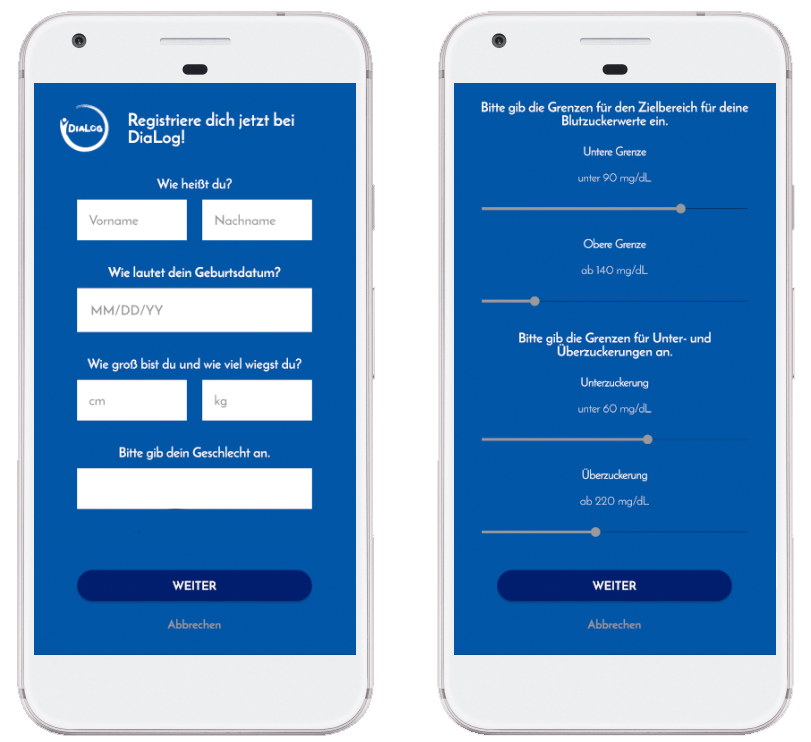
\includegraphics[width=0.7\textwidth]{images/DialogBox.png}
	\captionsetup{justification=centering}
	\caption{Dialog Boxes}
	\label{img:dialogbox}
\end{figure}
Hinzu kommen folgende Standards:
\begin{itemize}
	\item Use group boxes, embed all-caps titles in upper center of group box
	\item Order groups left to right, top to bottom according to natural order or expected frequency of use
	\item Always place the Weiter push button in the middle at the bottom and above the Abbrechen push button, all push buttons evenly apart
	\item Background color for fields:\newline
		\noindent\hspace*{30mm}Read-only - blue \newline
		\noindent\hspace*{30mm}Required - white \newline
		\noindent\hspace*{30mm}Optional - gray 
\end{itemize}

\subsection{Style Guide}
Um nun die Screen Design Standards zu vervollständigen, wird ein Style Guide erstellt. Dieser fügt dem User Interface folgende Kriterien hinzu:\\